\documentclass[10pt]{beamer}

\usepackage[T2A]{fontenc}
\usepackage[utf8]{inputenc}
\usepackage[russian]{babel}
\usepackage{multicol}
\usepackage{hyperref}
\usepackage{caption}
\usepackage{minted}
\usepackage{subcaption}
\setbeamertemplate{navigation symbols}{} %отключение значков
\setbeamertemplate{caption}[numbered]
\usetheme{Warsaw}
\setbeamertemplate{footline}{%
    \hspace{0.94\paperwidth}%
    \usebeamerfont{title in head/foot}%
    \insertframenumber\,/\,\inserttotalframenumber%
}
\newcommand{\pdiff}[2]{\frac{\partial #1}{\partial #2}}
\newcommand{\op}[1]{\mathop{\mathrm{#1}}}
\graphicspath{{pictures/}}
\begin{document}

\title{Цифровые методы синтеза аналоговых сигналов}
\author{Студент гр. 506: Вебер Д.С.\\Руководитель:  ст.пр. Уланов П.Н.}
\date{2024}
\institute{Алтайский государственный университет}


\frame{\titlepage}

\begin{frame}{Цель и задачи}
  \textbf{Цель работы:} реализовать метод синтеза на микроконтроллере.

  \textbf{Задачи:} 
  \begin{enumerate}
		\item Исследовать существующие методы синтеза аналоговых сигналов.
		\item Выбрать метод и освоить его алгоритм.
  \end{enumerate}
\end{frame}

\begin{frame}{Микроконтроллер}
  \begin{figure}
  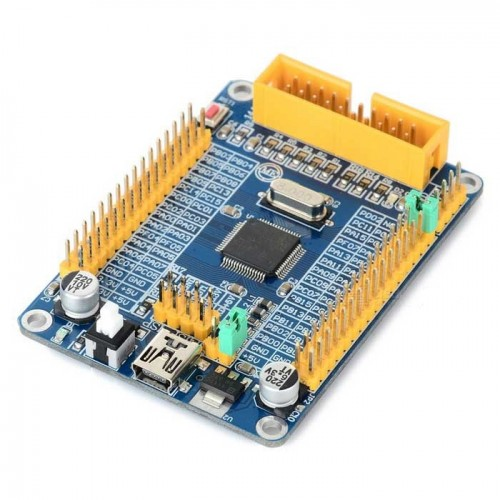
\includegraphics[width=0.45\textwidth]{stmka}
  \caption{Отладочная плата STM32F103RCT6.}
  \end{figure}
  Характеристики:
  \begin{itemize}
 	 \item Рабочее напряжение: 2 --- 3.6 В.
 	 \item Объём памяти: 256 Кб.
  	 \item Оперативная память: 48 Кб.
 	 \item Количество входов/выходов: 51.
 	 \item Цифро-аналоговый преобразователь: 2х12 б
  \end{itemize}
\end{frame}

\begin{frame}{Методы программной генерации сигнала}
Основные методы цифровой генерации сигналов:
  \begin{enumerate}
		\item Метод аппроксимации. 
		
		+: использование небольшой памяти. 
		
		---: затраты ресурсов на вычисления.
		\item Табличный метод.
		
		+: меньшее время и затрата ресурсов. 
		
		---: требуется больший объём памяти.
  \end{enumerate}


\end{frame}

\begin{frame}{Генерация отсчётов}
  \begin{figure}
  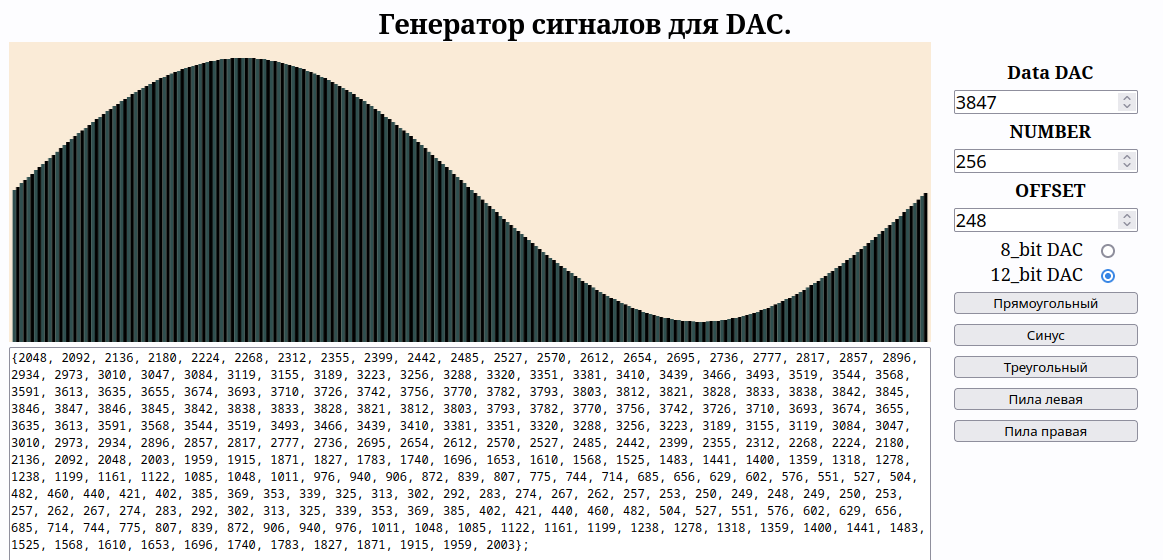
\includegraphics[width=1\textwidth]{lut}
  \caption{Таблица отсчётов.}
  \end{figure}
\end{frame}

\begin{frame}[containsverbatim]{ЦАП}
\begin{footnotesize}
  	Настройка ЦАП.
	\begin{minted}
	[
	frame=lines,
	framesep=2mm,
	baselinestretch=1.2,
	%fontsize=\footnotesize,
	linenos,
	breaklines
	]
	{text}
rcc_periph_clock_enable(RCC_GPIOA);
gpio_set_mode(GPIOA, GPIO_MODE_OUTPUT_2_MHZ, 
	GPIO_CNF_OUTPUT_ALTFN_PUSHPULL, GPIO5);
rcc_periph_clock_enable(RCC_DAC);
dac_enable(CHANNEL_2); 
	\end{minted}
	
	Загрузить значения в ЦАП
	\begin{minted}
	[
	frame=lines,
	framesep=2mm,
	baselinestretch=1.2,
	%fontsize=\footnotesize,
	linenos,
	breaklines
	]
	{text}
for (int i = 0; i < 256; i++)
{
	dac_load_data_buffer_single(lut[i], RIGHT12, CHANNEL_2);
}
	\end{minted}
\end{footnotesize}
\end{frame}


\begin{frame}{Моделирование DDS}
  \begin{figure}
  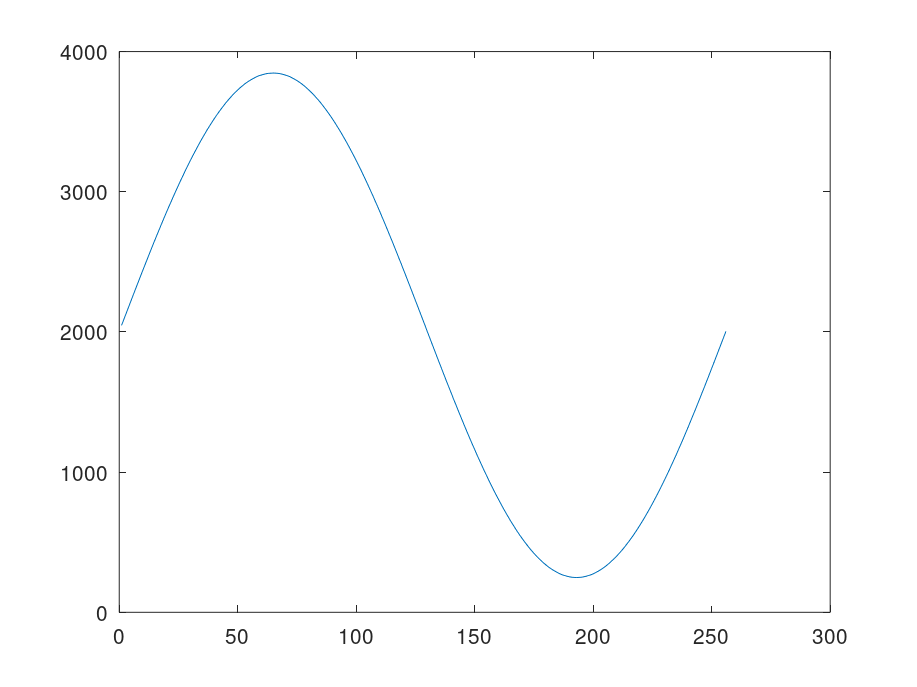
\includegraphics[width=0.9\textwidth]{tab_sin}
  \caption{Синтез синусоиды табличным методом.}
  \end{figure}
\end{frame}

\begin{frame}{Моделирование DDS}
  \begin{figure}
  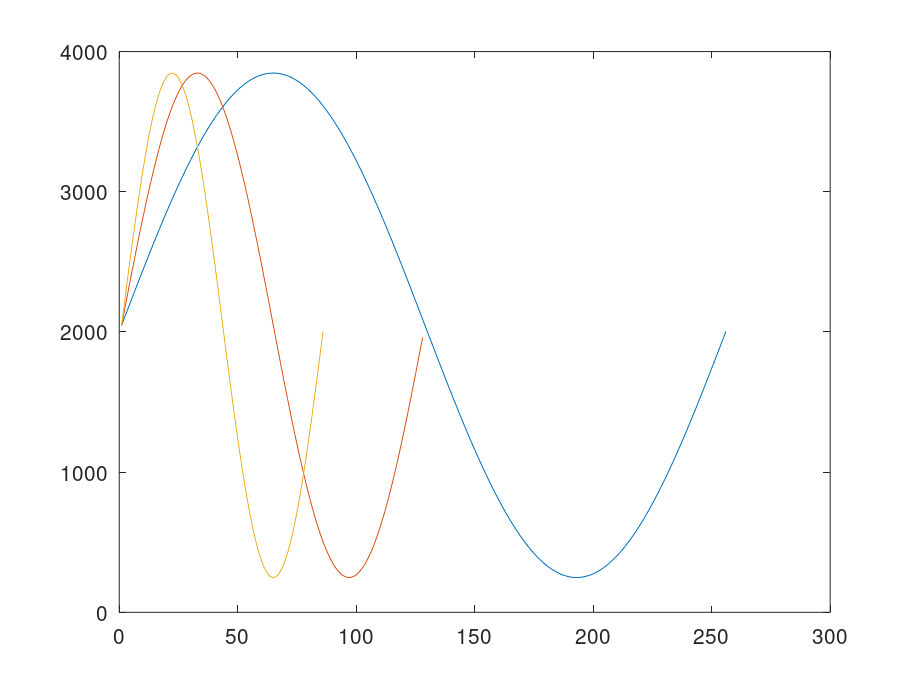
\includegraphics[width=0.9\textwidth]{tab_sin_s}
  \caption{Увеличение частоты сигнала.}
  \end{figure}
\end{frame}


\begin{frame}[containsverbatim]{Моделирование DDS}
	Для адресации используется аккумулятор фазы и код частоты. 
	
	Старшая часть аккумулятора фазы отвечает за адресацию ячейки в таблице отсчётов, а младшая за шаг в этой таблице. Размером же шага является код частоты.

	Аккумулятор фазы + Код частоты = Адрес отсчёта 
	
	0x0000 + 0x0100 = 0x0100

	0x0000 + 0x0200 = 0x0200
	
	0x0000 + 0x0080 + 0x0080 = 0x0100
		
\end{frame}

\begin{frame}{Моделирование DDS}
  \begin{figure}
  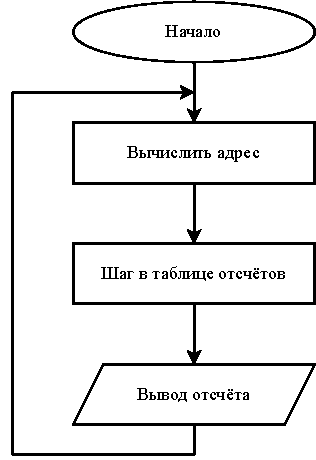
\includegraphics[width=0.45\textwidth]{dds_block}
  \caption{Алгоритм метода DDS.}
  \end{figure}
\end{frame}

\begin{frame}[containsverbatim]{Моделирование DDS}
\begin{footnotesize}
\begin{minted}
	[
	frame=lines,
	framesep=2mm,
	baselinestretch=1.2,
	%fontsize=\footnotesize,
	linenos,
	breaklines
	]
	{text}
int main() {
  uint16_t p_acc, p_step;
  uint8_t addr = 0; // адрес ячейки

  p_acc = 0;    // аккумулятор фазы
  p_step = 256; // код частоты

  while(1)
  {
    addr = p_acc >> 8; // выделение старшей части аккумулятора фазы
    p_acc += p_step;   // шаг
    printf("%d 0x%X\n", addr, sinus[addr]); // вывод отсчёта
  }

  return 0;
}
	\end{minted}
\end{footnotesize}
\end{frame}

\begin{frame}[containsverbatim]{Моделирование DDS}
Формирование отсчётов при коде частоты 256.
\begin{footnotesize}
\begin{minted}
	[
	frame=lines,
	framesep=2mm,
	baselinestretch=1.2,
	%fontsize=\footnotesize,
	linenos,
	breaklines
	]
	{text}
[kenny@desktop dds] gcc dds.c -o dds && ./dds
0 0x7F
1 0x82
...
254 0x79
255 0x7C
	\end{minted}
\end{footnotesize}
\end{frame}
	
	
\begin{frame}[containsverbatim]{Моделирование DDS}
Формирование отсчётов при коде частоты 512.
\begin{footnotesize}
\begin{minted}
	[
	frame=lines,
	framesep=2mm,
	baselinestretch=1.2,
	%fontsize=\footnotesize,
	linenos,
	breaklines
	]
	{text}
[kenny@desktop dds] gcc dds.c -o dds && ./dds
0 0x7F
2 0x85
...
252 0x73
254 0x79
	\end{minted}
\end{footnotesize}
\end{frame}
	

\begin{frame}[containsverbatim]{Моделирование DDS}
Формирование отсчётов при коде частоты 128.
\begin{footnotesize}
\begin{minted}
	[
	frame=lines,
	framesep=2mm,
	baselinestretch=1.2,
	%fontsize=\footnotesize,
	linenos,
	breaklines
	]
	{text}
[kenny@desktop dds] gcc dds.c -o dds && ./dds
0 0x7F
0 0x7F
1 0x82
1 0x82
...
254 0x79
254 0x79
255 0x7C
255 0x7C
	\end{minted}
\end{footnotesize}
\end{frame}

\begin{frame}{Реализация}
\begin{figure}
     \begin{subfigure}[H]{0.45\textwidth}
         \centering
         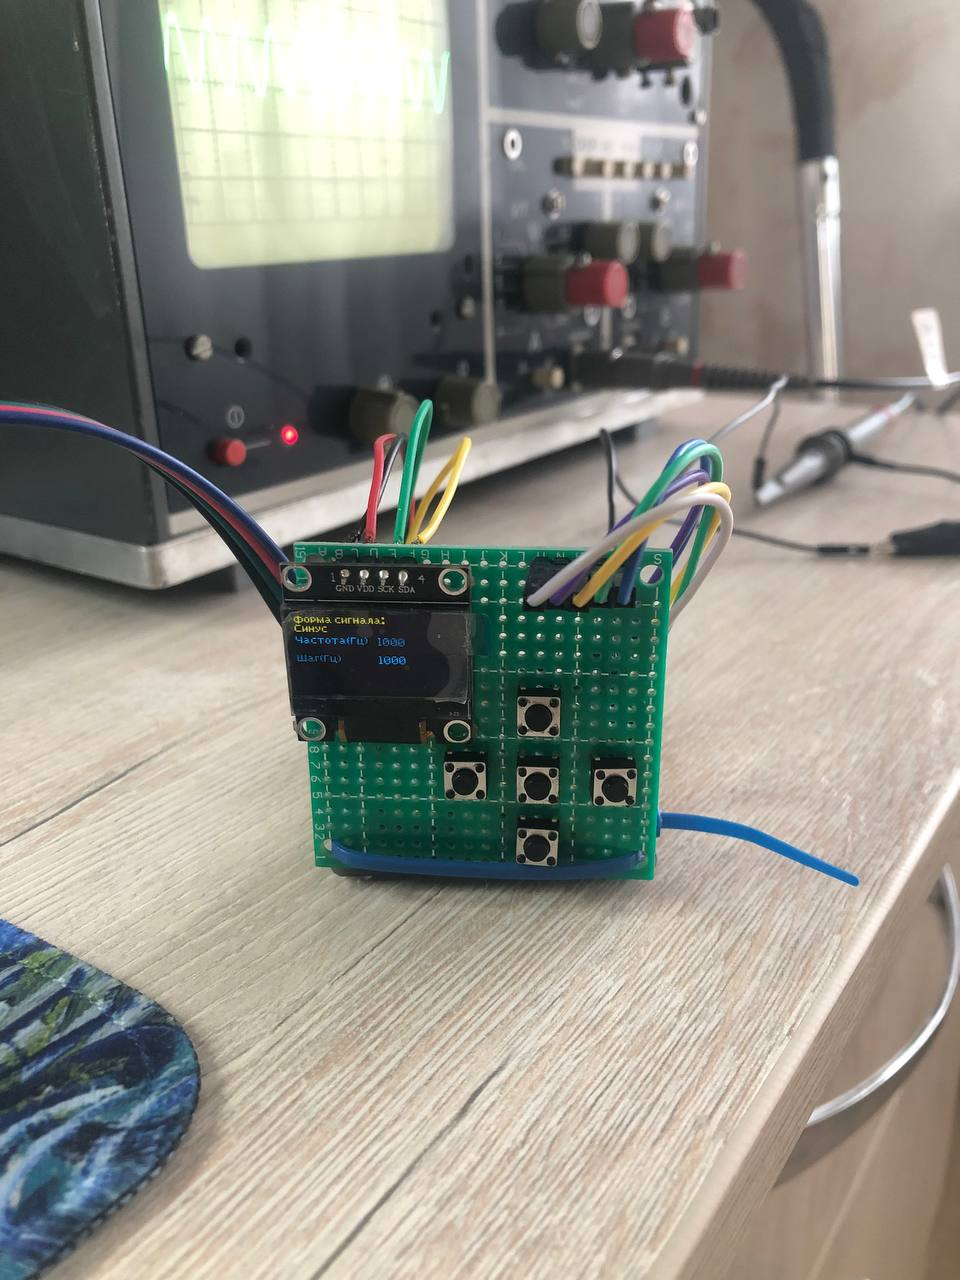
\includegraphics[width=\textwidth]{1}
         %\caption{Первый компьютер}
     \end{subfigure}
     \hfill
     \begin{subfigure}[H]{0.45\textwidth}
         \centering
         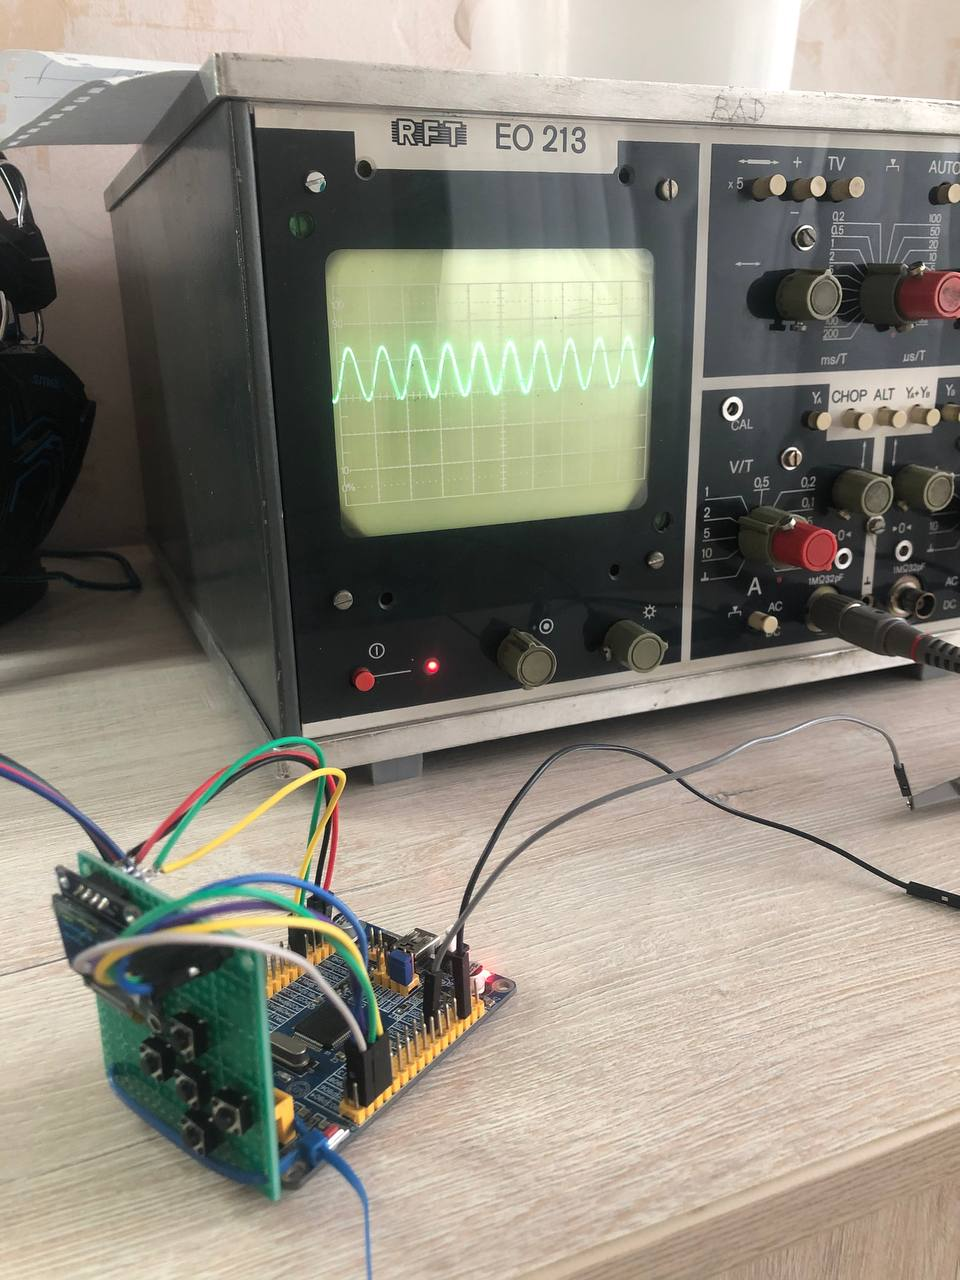
\includegraphics[width=\textwidth]{2}
         %\caption{Второй компьютер}
     \end{subfigure}
        \caption{Макет.}
\end{figure}
\end{frame}


\begin{frame}{Заключение}
	В ходе выполнения работы был реализовал метод синтеза на микроконтроллере.
	
	Были выполнены все поставленные задачи, а именно:
	\begin{enumerate}
		\item Исследованы существующие методы синтеза аналоговых сигналов.
		\item Выбран и освоен метод.
	\end{enumerate}
	
	Выбранный в результате исследования метод прямого цифрового синтеза сигнала применён в разработке программы генератора сигналов на микроконтроллере STM32.
\end{frame}

\begin{frame}{Спасибо за внимание!}
\url{https://github.com/lilbudek/stm32f1_libopencm3}
  \begin{figure}
  
\includegraphics[width=0.7\textwidth]{qr-code}
  \end{figure}
  
\end{frame}

\end{document}
